\chapter{Введение}
\label{sec:Chapter0} \index{Chapter0}

\section{Контекст проблемы}
На момент написания этой работы сложно переоценить влияние мобильных устройств на повседневную жизнь.
Смартфоны предоставляют огромный спектр возможностей, начиная от коммуникации и игр, заканчивая рабочими потребностями, навигацией и отслеживанием физического состояния человека.
Количество использующихся телефонов значительно преобладает над количеством ПК и ноутбуков.
Однако такой массовый характер был бы невозможен в отсутствии многообразия устройств на рынке.
Действительно, развитие технологий безусловно исходит из потребности в новых возможностях, однако финансирование этого развития поступает из уже существующих и отлаженных технологий.
Кроме того, только что изобретённой технологии требуется некоторое время, чтобы спрос на неё появился и вырос.
Исходя из этого, а также готовности потребителя пойти на компромисс между ценой за устройство и количеством и качеством предоставляемых им функций, представленные на рынке устройства коренным образом отличаются между собой.

\par
С другой стороны, имея такое разнообразие, разрабатывать приложения и отлаживать под каждое устройство было бы слишком дорогой задачей.
Чтобы решить эту проблему, вводится понятие виртуальной машины, то есть некоторого абстрактного вычислителя, способного исполнять инструкции из определённого набора, тем самым обеспечивая разработчиков приложений некоторым количеством гарантий.
Кажется очевидным, что этот подход аналогичен договорённости между программистами и разработчиками микропроцессоров в виде архитектуры системы команд и почти в той же степени необходим.
Главное отличие заключается в более высоком уровне абстракции, что позволяет переложить ответственность за управление ресурсами приложения, например выделение и освобождение памяти, на саму виртуальную машину, тем самым упрощая код и снижая требовательность к опыту разработчика.
В случае мобильных устройств, виртуальная машина рассматривается практически как неотъемлемая часть операционной системы, которая, помимо обеспечения гарантий разработчикам приложений, служит барьером безопасности для пользователей, устанавливающих и использующих самые разные приложения. 

\par
Высокоуровневость виртуальных машин позволяет выражать программы более компактно в сравнении с представлением в нативном коде.
В то же время, нативный код, полученный в результате анализа программы целиком, несравнимо быстрее поочерёдного исполнения инструкций виртуальной машины (интерпретации байткода).
Выходом из этой ситуации стало использование Just-In-Time компиляции, то есть генерации оптимизированного нативного кода для часто вызываемых функций, происходящей параллельно выполнению основного алгоритма.
Использование как классических оптимизаций (межпроцедурной оптимизации, раскрутки циклов) так и специфичных JIT-оптимизаций (профилирование типов в случае динамических языков) позволяет достичь производительности, нивелирующей накладные расходы вносимые этим уровнем абстракции.
В виртуальных машинах так же используется Ahead-Of-Time компиляция, производящаяся до запуска приложения.
Это позволяет избежать излишних затрат энергии при повторных запусках приложений связанных с JIT-компиляцией, скомпилировать большее количество методов, и, возможно, применить большее количество оптимизаций, тем самым экономя заряд батареи мобильных устройств, ускоряя время запуска и улучшая производительность приложения ценой хранения результатов компиляции (AOT-файлов) на устройстве.

\par
Очевиден тот факт, что множество приложений в своих подзадачах часто используют идентичные алгоритмы, такие как сортировка, работа со строками и т. д., и что множественная имплементация того или иного алгоритма ведёт к практической сложности поддержки такого кода.
Ввиду этого, многие алгоритмы, оптимизированные с целью быть приемлимо эффективными для самых различных нагрузок, образуют стандартную библиотеку языка и поставляются вместе с виртуальной машиной.
Будучи часто переиспользуемой, стандартная библиотека AOT-компилируется и хранится на устройстве, что позволяет любому приложению гарантировано использовать оптимизированный нативный код, не совершая излишнюю работу по JIT-компиляции.

\par
Выпуская огромное количество устройств, запуск AOT-компиляции стандартной библиотеки на каждом из них был бы нерационален и сопровождался бы ощутимыми издержками производства.
Их можно избежать путём единовременной компиляции и последующей загрузки полученного образа на устройства, например при прошивке.
Для подготовки образа виртуальной машины и операционной системы используется специальный набор утилит, включающий в себя кросс-компилятор и опции компиляции, который работает на отличной от целевого устройства платформе и генерирующий исполняемые файлы в виде нативного кода целевого устройства.
Для такого набора утилит принят термин таргет-тулчейн, в то время как для аналогичного набора утилит, предназначенных для получения исполняемых файлов для той же платформы на которой они и были сгенерированы, используется термин хост-тулчейн.

\par
Однако, таргет-тулчейн не подходит для непосредственной подготовки AOT-файла стандартной библиотеки.
Это связано с тем, что стандартная библиотека рассчитана на исполнение в среде виртуальной машины, отличающейся от окружения создаваемого операционной системой и может проявляться в том, что тулчейн-компилятор и AOT-компилятор виртуальной машины могут использовать разное соглашение о вызовах.
Поэтому приобретает смысл вопрос о кросс-компиляторе в терминах виртуальной машины, что на самом деле означает возможность генерации AOT-файлов виртуальной машины для определённого устройства на другой платформе, например на сервере. Эта задача имеет множество тонкостей, одной из которых посвящена данная работа - проблема зависимости некоторых численных значений от платформы (платформо-зависимых констант).
Наиболее ярким примером является размер указателя.
Однако в этом случае зависимость от платформы достаточно легко <<предсказать>>: на AMD64-совместимой платформе это скорее всего 8 байт, а на ARM32 - 4.
Другим, более трудноразрешимым и содержательным примером является смещение до полей в структурах данных.
Даже в процессе компиляции на одной и той же платформе одним и тем же компилятором, в зависимости от опций компиляции результат может быть различным.
В последующих главах излагается подробное описание этой проблемы, на примере абстрактной виртуальной машины демонстрируется один из источников таких значений, а также предлагается решение, основанное на использовании таргет-тулчейна, нашедшее применение в некоторой виртуальной машине.
Как будет показано в дальнейшем, эта имплементация отличается высоким уровнем автоматизации и масштабируемости, делающей её малозаметной и лёгкой в использовании.
Кроме того, помимо основной функции, она вносит дополнительную степень верификации AOT-файлов.

\section[Описание проблемы]{Описание проблемы на практическом примере}
Рассмотрим более подробно язык программирования, который поддерживает какая-либо представляющая интерес виртуальная машина, реализованная, для определённости, на языке C++.
Положим также, что в нём существуют некоторые встроенные типы, это могут быть числа, строки массивы, словари и т.д., а операции с этими сущностями, например их создание, модификация, получение внутреннего состояния, выражаются в специальных инструкциях виртуальной машины.
Тогда при исполнении программы созданию массива будет соответствовать выполнение некой инструкции \textit{newarray}, а получению длины этого массива -- выполнение \textit{arraylength} (рис. 2.1).

\begin{figure}[H]
    \centering
    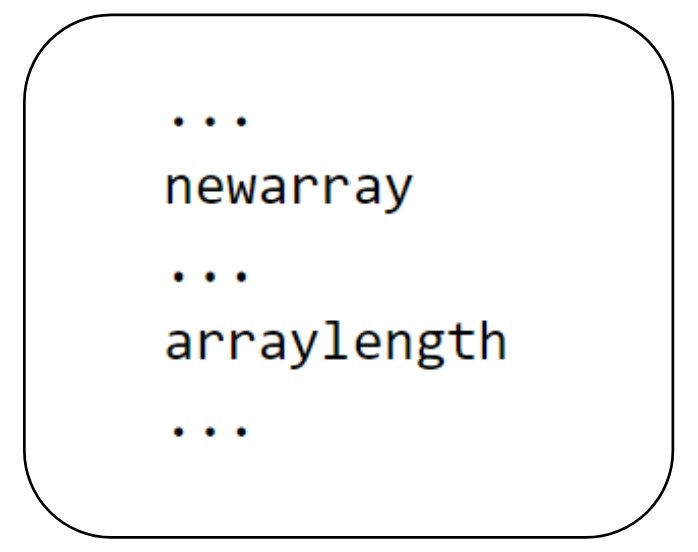
\includegraphics[scale=0.7]{bytecodes_array.jpg}
    \caption{Пример инструкций в программе}
\end{figure}

С другой стороны, каждый встроенный тип находит отражение в некотором C++-классе. При этом, при исполнении инструкции \textit{newarray} будет происходить аллокация экземпляра этого класса, а при исполнении \textit{arraylength} будет произведено чтение поля \textit{size\_} одного из экземпляров (рис. 2.2).

\begin{figure}[H]
    \centering
    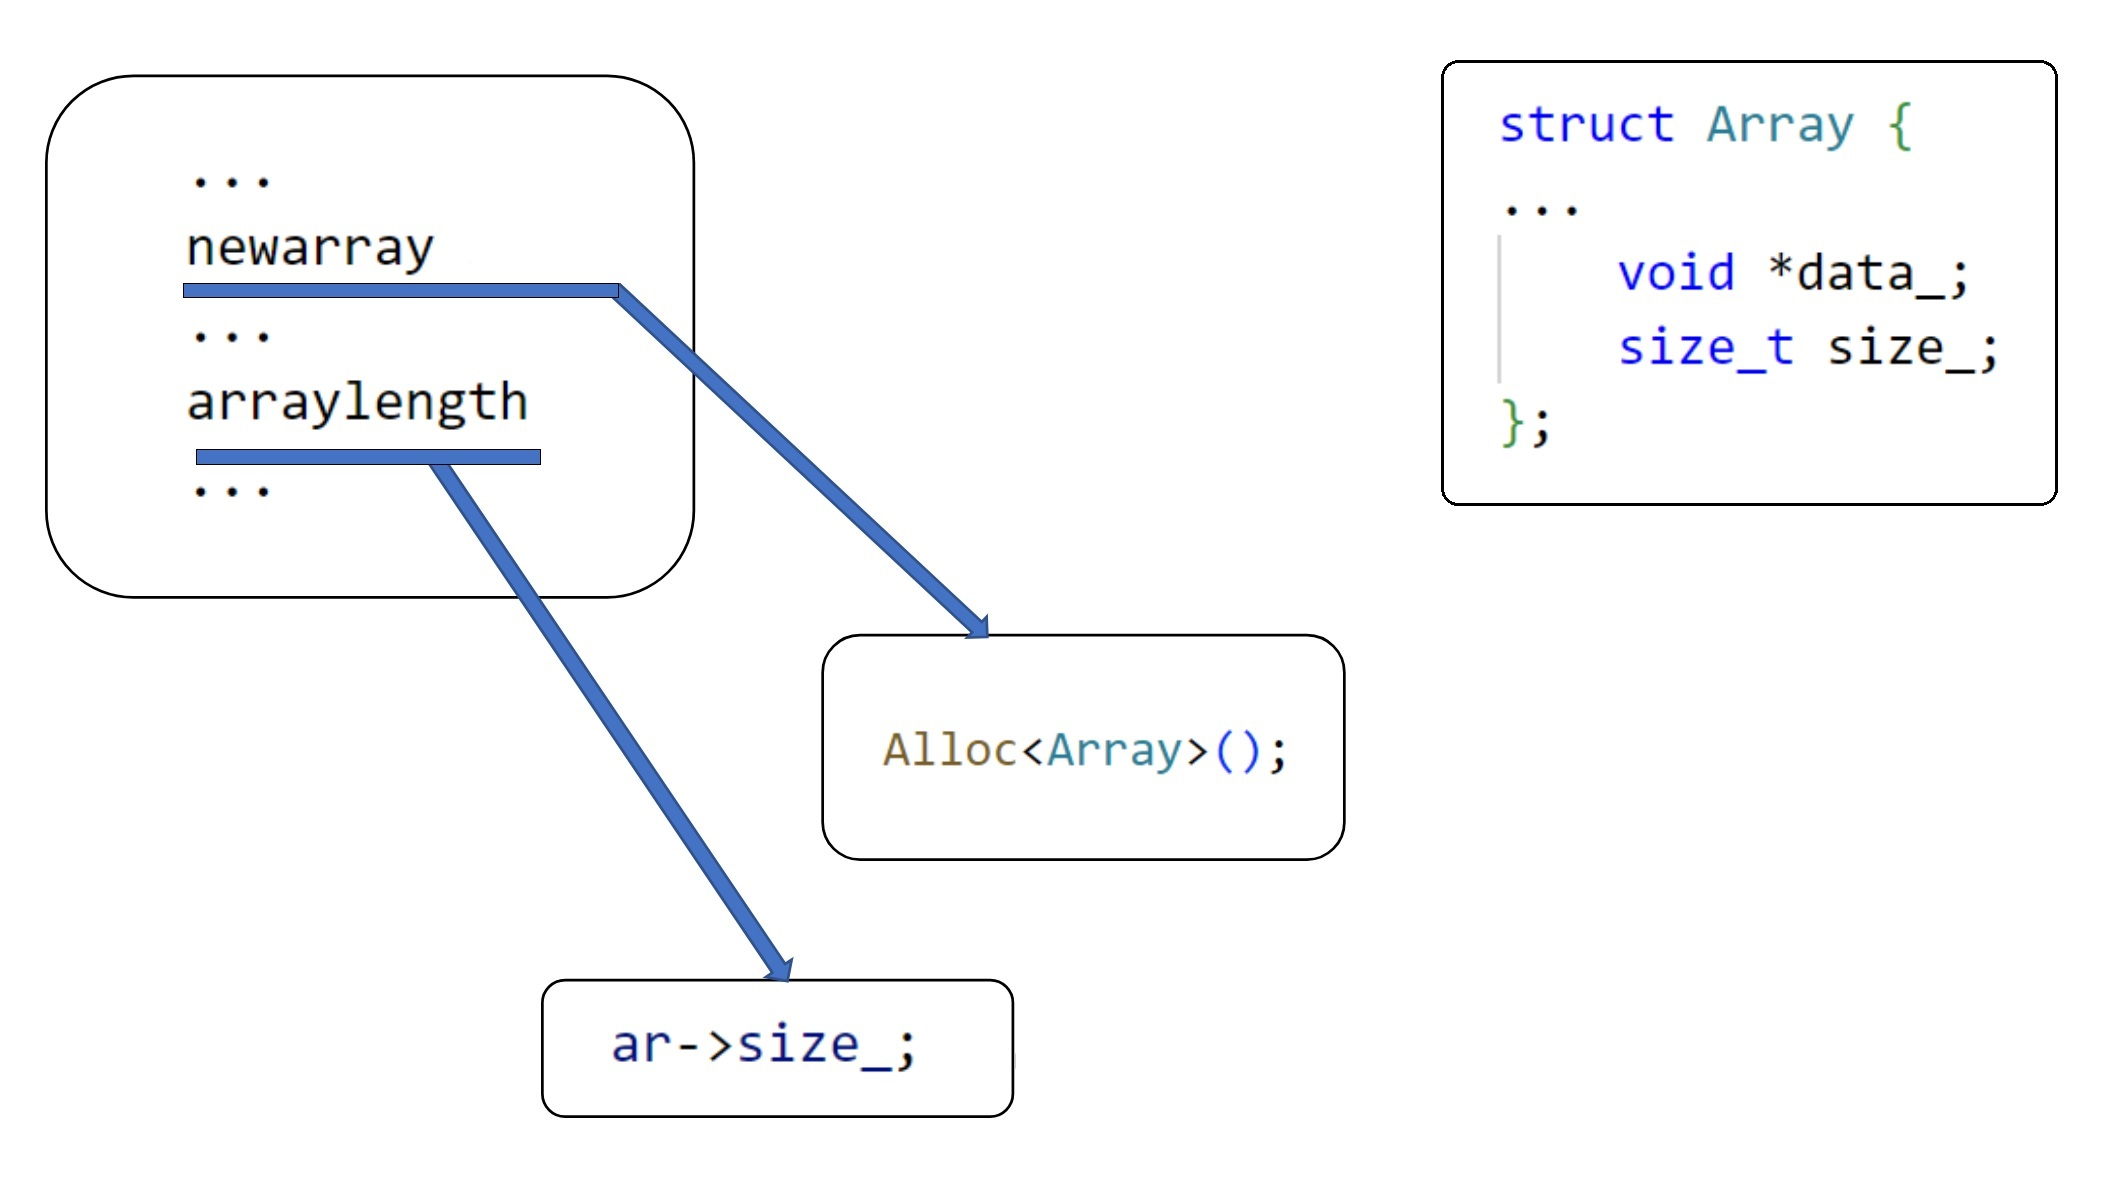
\includegraphics[scale=0.5]{mirror_class.jpg}
    \caption{Реализация семантики языка}
\end{figure}

В нативном формате обращение к этому полю будет выражено в виде машинной инструкции загрузки по указателю с константным смещением.
Возвращаясь к кросс-компилятору виртуальной машины, эта инструкция будет создана на финальном этапе, кодогенерации, из соответствующей инструкции промежуточного представления.
Фактически, эта инструкция промежуточного представления абстрагирует бинарный формат машинной инструкции загрузки по смещению конкретной архитектуры, отделяя зависимость от платформы.
Однако, такой абстракции для отделения оказывается недостаточно.
\par
Дело в том, что смещение до поля класса (эквивалентное в рассматриваемой ситуации смещению в инструкции загрузки), в общем случае, зависит от платформы.
Это может происходить по разным причинам, например -- из-за зависимости размера какого-либо элемента структуры данных от платформы, выравнивания по разным адресам.
Так, рассматриваемое ранее смещение до поля \textit{size\_} структуры \textit{Array} на 64-битной архитектуре AMD64 будет равно 8 байтам, хотя на архитектуре ARM32 -- 4.
Если упустить из рассмотрения этот факт, то кросс-компилятор виртуальной машины, запущенный на AMD64-сервере, при генерации ARM32-инструкций будет использовать соответствующее текущей платформе значение смещения.
Тогда, при запуске такого кода на ARM32-телефоне, исполнение такой инструкции приведёт к некорректному поведению и будет являться программной уязвимостью.
Вопрос корректности и безопасности генерируемого кода является первостепенным в процессе компиляции, что подчёркивает значимость этой проблемы.
\par
Можно выделить два подхода, позволяющие разрешить этот конфликт: первый -- сделать смещения для всех платформ одинаковыми, второй -- каким-либо образом сообщать компилятору значение константы на платформе, для которой происходит компиляция. Данная работа посвящена главным образом реализации второго из них, однако в следующих главах также производится сравнение этих подходов, обосновывающее этот выбор.

\section{Терминология}
Для дальнейшего повествования удобно ввести следующие определения.

\begin{itemize}
    \item
        \textit{Тулчейн} -- набор утилит, позволяющий транслировать C++-программы в некоторый бинарный код.
    \item
        \textit{Платформа} -- предполагаемое тулчейном окружение, в котором будет исполняться сгенерированный им код. Подразумевается, что каждая платформа в достаточной степени однозначно определяется некоторым тулчейном. В качестве синонима, в данной работе может также использоваться термин \textit{архитектура}.
    \item
        \textit{Хост-тулчейн} -- тулчейн предназначенный для генерации кода, совместимого с той же платформой, на которой и генерируется.
    \item
        \textit{Таргет-тулчейн} -- тулчейн предназначенный для генерации кода, совместимого с платформой отличной от той, на которой был сгенерирован.
    \item
        \textit{Платформо-зависимая константа} -- именованное, определённое в терминах C++ константное выражение, численное значение которой каким-либо образом зависит от платформы. Под этим термином может пониматься как множество численных значений какой-либо величины на всех платформах, так и само значение на какой-то конкретной платформе.
    \item
        \textit{Гостевая константа} -- значение платформо-зависимой константы, соответствующее некоему таргет-тулчейну.
\end{itemize}

\newpage